\subsection{Long vowel headedness}
Whether long vowels are head-final or head-initial determines
if a language allows super-heavy Rhymes of the form \ctx{VVCC},
i.e. whether Rhymes are \TODO{}
allowed to dominate up to three skeletal slots instead of only two.

If long vowels are head-initial (\cref{fig:long vowels:init}),
the second Nucleus has to be licensed by a following nucleus.
If it fails to be licensed, a short vowel surfaces.%
\footnote{\Citeauthor{scheer2004} \tr{gleichsetzen} \TODO{}}

Otherwise (\cref{fig:long vowels:fin}),
if the second Nucleus is the head of the long vowel,
it licenses the preceding Nucleus and the long vowel is self-licensing,
i.e. it doesn't need any external support.

\TODO{das doppelt sich jetzt mit \cref{fig:intro:longV}}
\begin{figure}[h]
  \centering
  \begin{subfigure}{.49\textwidth}
    \centering
    \begin{structure}{}
      \drawCV{1}
      \C{C}
      \V{V}
      \emptyC
      \emptyV
      \draw[dashed] (pV1) -- (V2);
      \draw[<-] (V2.north) -- ++(0,0.2) -- node[above]{Lic} ++(1,0);
    \end{structure}
    \caption{alternating long vowels are head-initial}
    \label{fig:long vowels:init}
  \end{subfigure}
  \hfill
  \begin{subfigure}{.49\textwidth}
    \centering
    \begin{structure}{}
      \drawCV{1}
      \C{C}
      \longV{V}
    \end{structure}
    \caption{non-alternating long vowels are head-final}
    \label{fig:long vowels:fin}
  \end{subfigure}
  \captionsource{long vowel headedness}{\cite[p.~267]{scheer2004}}
\end{figure}

\paragraph{In german:}
Since there are no alternations in vowel length in German,
long vowels are self-licensing and therefore head-final.

\TODO{Are super-heavy Rhymes allowed? (VVCC). Doesn't this contradict the statement above of "up to three sceletal slots"?}
Schon, mit \ex{Obst} \ti{[o:pst]} sogar VVCCC!
(Angst, sanft, sonst, Arzt \ti{[artst]})


\subsection[Schwa]{Schwa\footnotemark}
\label{subsec:params:schwa}
  \footnotetext{
    In \cite{scheer2004}, \enquote{schwa} is defined phonologically
    as a vowel alternating with zero, with the added remark that for
    languages like German this coincides with its phonetic
    reality: \textquote[{\cite[][p.~564]{scheer2004}}]{the alternating
    vowel is phonetically central and thus overtly deserves the name
    \enquote{schwa}}.
  }
Schwa does govern
\TODO{why}

Schwa does not license: \cite{scheer2004} analyzes the distribution
of \textipa{[N]} vs. \textipa{[Ng]} as an underlying \textipa{/Ng/}
where the \textipa{/g/} only surfaces if it is licensed.
In this analysis, three contexts are examined:

\begin{figure}[h]
  % \centering
  \captionsetup[subfigure]{
    labelformat=simple,        % no braces around label
    labelsep=period,           % period after label
    justification=raggedright, % align left
    singlelinecheck=false,     % disable automatic centering of single-line captions
    position=top,              % subcaptions are above their content
  }
  \begin{subfigure}[T]{.5\textwidth}
    \caption{\ti{[N]} in closed syllables}
    \label{fig:ng:closed syllable}
    \begin{structure}{Pi\textbf{ng}po\textbf{ng} \ti{[pINpON]}}
      \drawCV{5}
      \C{p}
      \V{\ti{I}}
      \Ng[nolic]
      \emptyV[gov]
      \C{p}
      \V{\ti{O}}
      \Ng[nolic]
      \fen
    \end{structure}
  \end{subfigure}
  \hfill
  \begin{subfigure}[T]{.45\textwidth}
    \caption{\ti{[N]} before schwa}
    \label{fig:ng:before schwa}
    \begin{structure}{I\textbf{ng}e \ti{[PIN@]}}
      \drawCV{2}
      \C{\ti{P}}
      \V{\ti{I}}
      \Ng[nolic]
      \V{\textschwa}
    \end{structure}
  \end{subfigure}

  \vspace{1.5em}
  \begin{subfigure}[T]{\textwidth}
    \caption{\ti{[Ng]} before full vowels (i.e. that are different from schwa)}
    \label{fig:ng:before full vowel}
    \begin{structure}{I\textbf{ng}o \ti{[PINgo:]}}
      \drawCV{2}
      \C{\ti{P}}
      \V{\ti{I}}
      \Ng[lic]
      \V{o}
    \end{structure}
  \end{subfigure}

  \captionsource{German: schwa does not license}{\cite[p.~580]{scheer2004}}
\end{figure}

Since \textipa{/g/} doesn't surface before schwa it is concluded
that schwa doesn't license in German.%
\footnote{\TODO{Licensing of Nuclei unclear:
  \q[p.~660]{scheer2004}{%
    Since there is no Closed Syllable Shortening in this
    language, the status of schwa with respect to
    internuclear Licensing lies beyond our control.
    However, the prediction is that German would behave
    like Czech (see §430) if there were such a process.
    Since schwa is unable to license Onsets,
    it should not be in a position to license Nuclei either.
    Therefore long vowels ought not to occur before schwa.}
}}

\subsection{FEN}
\marknote{FEN hier ausschreiben?}
\label{subsec:params:fen}
The lateral actorship of FEN can be determined by their effect
on preceeding Nuclei and Onsets. \Cref{tab:params_fen} lists
all possible combinations.

\begin{table}
  \centering
  \begin{tabular}{c l | c c | c}
    & & \multicolumn{2}{c|}{effect on preceeding Nuclei:} & effect on preceding Onsets: \\
    &        & existence & vowels in final     & word-final consonants and \\
    & & of \ctx{...RT\#} & and internal        & internal Codas \\ 
    & FEN can   &        & closed syllables    & \\
  \cline{2-5}
  a.& + license &     &                        & contrast \\
    & + govern  & yes & contrast:              & word-final consonant = inter \\
    &           &     & vowel in \ctx{\_C\#} = & vocalic \\
  \cdashline{2-3}\cdashline{5-5}
  b.& + license &     & vowel in an            & contrast \\
    & - govern  & no  & open syllable          & word-final consonant = post- \\
    &           &     &                        & Coda \\
  \cline{2-5}
  c.& - license &     &                        & contrast \\
    & + govern  & yes &                        & word-final consonant is in the \\
    &           &     & behaves alike          & weakest possible situation \\
  \cdashline{2-3}\cdashline{5-5}
  d.& - license & \multirow{2}{*}{no} &        & \multirow{2}{*}{behaves alike} \\
    & - govern  &     &                        & \\
  \cline{2-5}
  \end{tabular}
  \caption[Parameters of FEN]{%
    Parameters of FEN
    {\small(from \cite[p.~545]{scheer2004})}}
  \label{tab:params_fen}
\end{table}

Final devoicing illustrates that word-final consonants behave like Codas.
It isn't clear whether they are weaker than internal Codas, either way the
parametrization of german FEN must be one of the lower two and in consequence
FEN are proper licensors.

Words like \ex{Hast}, \ex{Hand} and \ex{Kiosk} demonstrate that there
are \ctx{...RT\#} words in German, therefore FEN must be able to govern.


\subsection{Initial CV}
One indicator for the presence of the initial CV are coocurrence restrictions
on initial consonant clusters:
Since only \ctx{\#TR} clusters can contract Infrasegmental Government,
the empty Nucleus enclosed by a \ctx{\#RT} cluster can't possibly govern
the empty Nucleus of the initial CV.

scheer2012: p.~188:
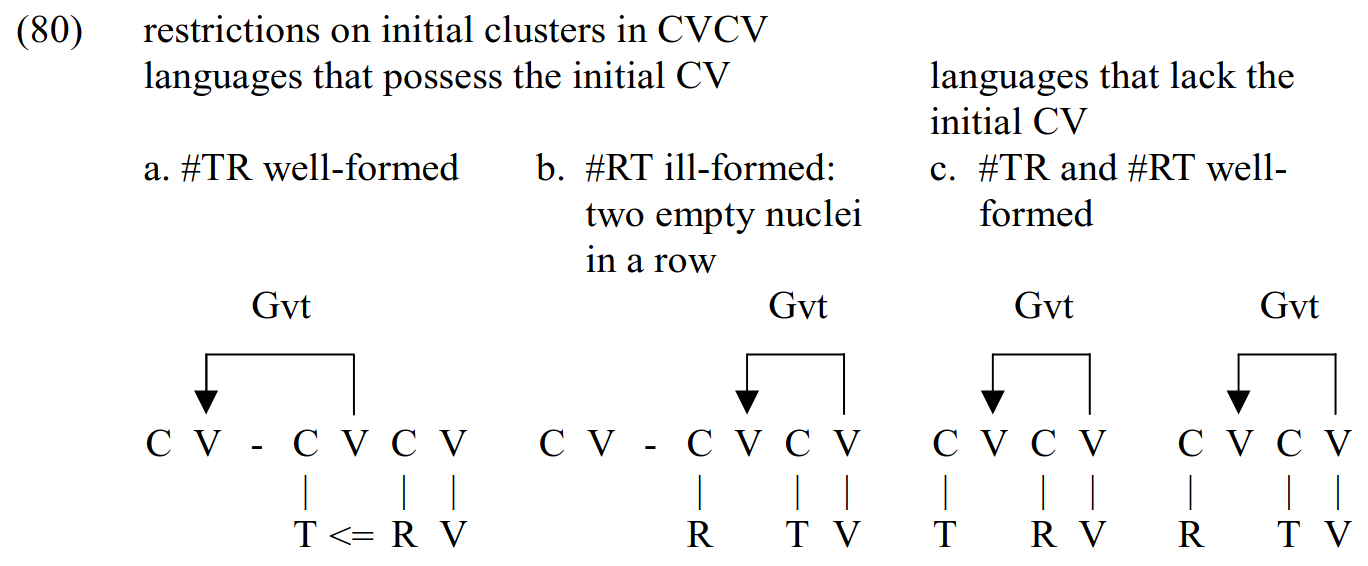
\includegraphics[width=.5\textwidth]{figures/scheer2012_initial-cv-initial-clusters.png}

Therefore, \CVCV predicts languages where \ctx{\#RT} is ill-formed to have
the initial CV.

In German, the only initial \ctx{\#RT} clusters are ones that start with
\textipa{[s]} or \textipa{[S]}, both of which are exceptional \TODO{}

\TODO{RT ist ja gar nicht Plosiv+... sondern R schließt ja auch Frikative ein.
Funktioniert IG auch zwischen Plosiv+Frikativ Sequenzen?}


\subsection{Stress assignment}
\TODO{kommt raus. Erwähnen?}